\let\lesson\undefined
\newcommand{\lesson}{\phantomlesson{Bài 11.}}
\setcounter{section}{2}
\section{Bài tập trắc nghiệm}
\begin{enumerate}[label=\bfseries Câu \arabic*:,leftmargin=1.5cm]
		\item \mkstar{1}
	
	
	{Một vật trượt trên một mặt phẳng, khi tốc độ của vật tăng thì hệ số ma sát giữa vật và mặt phẳng
		\begin{mcq}(2)
			\item không đổi.
			\item giảm xuống.
			\item tăng rồi giảm.
			\item giảm rồi tăng.
		\end{mcq}
	}
	
	\hideall
	{	\textbf{Đáp án: A.}
		
		Một vật trượt trên một mặt phẳng, khi tốc độ của vật tăng thì hệ số ma sát giữa vật và mặt phẳng không đổi.	
	}
	\item \mkstar{1}
	
	
	{Chiều của lực ma sát nghỉ
		\begin{mcq}
			\item ngược chiều với vận tốc của vật.
			\item ngược chiều với gia tốc của vật.
			\item ngược chiều với thành phần ngoại lực song song với mặt tiếp xúc.
			\item vuông góc với mặt tiếp xúc.
		\end{mcq}
	}
	\hideall
	{	\textbf{Đáp án: C.}
		
		Chiều của lực ma sát nghỉ ngược chiều với thành phần ngoại lực song song với mặt tiếp xúc.
		
	}
	
	\item \mkstar{1}
	
	
	{Chọn phát biểu \textbf{sai}.
		\begin{mcq}
			\item Lực ma sát trượt xuất hiện khi vật này trượt trên vật khác.
			\item Hướng của ma sát trượt tiếp tuyến với mặt tiếp xúc và ngược chiều chuyển động.
			\item Hệ số ma sát lăn luôn bằng hệ số ma sát trượt.
			\item Viên gạch nằm yên trên một mặt phẳng nghiêng vì chịu tác dụng của lực ma sát nghỉ.
		\end{mcq}
	}
	
	\hideall
	{	\textbf{Đáp án: C.}
		
		Với cùng một cặp vật liệu tiếp xúc, hệ số ma sát lăn rất nhỏ so với hệ số ma sát trượt.
	}
	\item \mkstar{2}
	
	
	{Một người kéo một thùng hàng chuyển động, lực tác dụng vào người đó giúp người đó chuyển động về phía trước là
		\begin{mcq}(2)
			\item lực của người kéo tác dụng vào đất.
			\item lực của thùng hàng tác dụng vào người kéo.
			\item lực của người kéo tác dụng vào thùng hàng.
			\item lực ma sát giữa mặt đất và chân người kéo.
		\end{mcq}
	}
	
	\hideall
	{	\textbf{Đáp án: D.}
		
		Một người kéo một thùng hàng chuyển động, lực tác dụng vào người đó giúp người đó chuyển động về phía trước là lực ma sát giữa mặt đất và chân người kéo.
	}
	\item \mkstar{2}
	
	
	{Một vật có khối lượng 5 tấn đang chuyển động trên đường nằm ngang có hệ số ma sát giữa vật và mặt đường là $\SI{0.2}{}$. Lấy $g=\SI{10}{m/s^2}$. Độ lớn của lực ma sát là
		\begin{mcq}(4)
			\item $\SI{1000}{N}$.
			\item $\SI{10000}{N}$.
			\item $\SI{100000}{N}$.
			\item $\SI{1000000}{N}$.
		\end{mcq}
	}
	
	\hideall
	{	\textbf{Đáp án: B.}
		
		Độ lớn của lực ma sát:
		$$F_\text{ms} = \mu m g = \SI{10000}{N}$$
	}
	\item \mkstar{3}
	
	
	{Một toa tàu có khối lượng 80 tấn chuyển động thẳng đều dưới tác dụng của lực kéo nằm ngang $F=\SI{6e4}{N}$. Lấy $g=\SI{10}{m/s^2}$. Hệ số ma sát giữa tàu và đường ray là
		\begin{mcq}(4)
			\item $\SI{0.075}{}$.
			\item $\SI{0.06}{}$.
			\item $\SI{0.02}{}$.
			\item $\SI{0.08}{}$.
		\end{mcq}
	}
	
	\hideall
	{	\textbf{Đáp án: A.}
		
		Tàu chuyển động thẳng đều khi
		$$F_\text{ms} = F = \mu mg \Rightarrow \mu = \SI{0.075}{}$$
	}
	
	\item \mkstar{3}
	
	
	{Người ta đẩy vật nặng $\SI{35}{kg}$ chuyển động theo phương nằm ngang bằng một lực có độ lớn $\SI{210}{N}$. Biết hệ số ma sát trượt giữa vật và mặt phẳng là $\SI{0.4}{}$. Lấy $g=\SI{10}{m/s^2}$. Gia tốc của vật là
		\begin{mcq}(4)
			\item $\SI{2}{m/s^2}$.
			\item $\SI{2.4}{m/s^2}$.
			\item $\SI{1}{m/s^2}$.
			\item $\SI{1.6}{m/s^2}$.
		\end{mcq}
	}
	
	\hideall
	{	\textbf{Đáp án: A.}	
		
		Tổng hợp lực tác dụng lên vật:
		$$\Sigma F= F-F_\text{ms} = F - \mu mg = \SI{70}{N}$$
		
		Áp dụng định luật II Newton:
		$$a=\dfrac{F}{m} = \SI{2}{m/s^2}$$
		
		Vậy $l_2 = \SI{27.5}{cm}$.
	}
	\item \mkstar{3}
	
	
	{Một vật có khối lượng $m=\SI{15}{kg}$ được kéo trượt trên mặt phẳng nằm ngang bằng lực kéo $F=\SI{45}{N}$ (theo phương ngang) từ trạng thái nghỉ. Cho hệ số ma sát trượt giữa vật và mặt phẳng nằm ngang là $\mu = \SI{0.05}{}$. Lấy $g=\SI{10}{m/s^2}$. Tính quãng đường vật đi được sau $\SI{5}{s}$ kể từ lúc bắt đầu chuyển động.
		\begin{mcq}(4)
			\item $S=\SI{50}{m}$.
			\item $S=\SI{75}{m}$.
			\item $S=\SI{12.5}{m}$.
			\item $S=\SI{31.25}{m}$.
		\end{mcq}
	}
	
	\hideall
	{	\textbf{Đáp án: D.}	
		
		Tổng hợp lực tác dụng lên vật:
		$$\Sigma F= F-F_\text{ms} = F - \mu mg = \SI{37.5}{N}$$
		
		Áp dụng định luật II Newton:
		$$a=\dfrac{F}{m} = \SI{2.5}{m/s^2}$$
		
		Vậy $S=\dfrac{1}{2}at^2 = \SI{31.25}{m}$.
	}
	\item \mkstar{3}
	
	
	{Một đầu máy tạo ra lực kéo để kéo một toa xe có khối lượng 5 tấn chuyển động với gia tốc $\SI{0.3}{m/s^2}$. Biết lực kéo của động cơ song song với mặt đường và hệ số ma sát giữa toa xe và mặt đường là $\SI{0.02}{}$. Lấy $g=\SI{10}{m/s^2}$. Lực kéo của đầu máy tạo ra là
		\begin{mcq}(4)
			\item $F=\SI{4000}{N}$.
			\item $F=\SI{3200}{N}$.
			\item $F=\SI{2500}{N}$.
			\item $F=\SI{5000}{N}$.
		\end{mcq}
	}
	
	\hideall
	{	\textbf{Đáp án: C.}	
		
		Áp dụng định luật II Newton:
		$$\Sigma F = ma = \SI{1500}{N}$$
		
		Lực kéo của đầu máy toa xe:
		$$\Sigma F= F-F_\text{ms} \Rightarrow F = \Sigma F + \mu mg = \SI{2500}{N}$$
	}
	\item \mkstar{4}
	
	
	{Một khúc gỗ khối lượng $\SI{2}{kg}$ đặt trên sàn nhà. Người ta kéo khúc gỗ bằng một lực $F$ hướng chếch lên và hợp với phương nằm ngang một góc $\alpha=30^\circ$. Khúc gỗ chuyển động nhanh dần đều với gia tốc $\SI{1}{m/s^2}$ trên sàn. Biết hệ số ma sát trượt giữa gỗ và sàn là $\SI{0.2}{}$. Lấy $g=\SI{10}{m/s^2}$. Giá trị của $F$ là
		\begin{mcq}(4)
			\item $\SI{4.24}{N}$.
			\item $\SI{4.85}{N}$.
			\item $\SI{6.21}{N}$.
			\item $\SI{5.12}{N}$.
		\end{mcq}
	}
	
	\hideall
	{	\textbf{Đáp án: C.}
		
		Độ lớn của lực $F$ trên phương thẳng đứng:
		$$F_y = F \sin \alpha = \dfrac{F}{2}$$
		
		Độ lớn của phản lực:
		$$N=mg-F_y $$
		
		Độ lớn của lực ma sát:
		$$F_\text{ms} = \mu N$$
		
		Vật chuyển động nhanh dần đều, áp dụng định luật II Newton:
		$$F \cos \alpha - F_\text{ms} = ma \Rightarrow F \cos \alpha - \mu (mg - F \sin \alpha) \Rightarrow F = \SI{6.21}{N} $$
		
	}
\end{enumerate}
\section{Bài tập tự luận}
\begin{enumerate}[label=\bfseries Bài \arabic*:,leftmargin=1.5cm]
		\item \mkstar{1}
	
	{
		Nêu những đặc điểm của lực ma sát trượt, lực ma sát nghỉ.
	}
	
	\hideall{
		
		Những đặc điểm của lực ma sát trượt:
		\begin{itemize}
			\item Xuất hiện ở mặt tiếp xúc của vật đang trượt trên một bề mặt;
			\item Có hướng ngược hướng của vận tốc;
			\item Có độ lớn tỉ lệ với độ lớn của áp lực, không phụ thuộc vào diện tích tiếp xúc và tốc độ của vật;
			\item Biểu thức: $F_\text{mst} = \mu_\text t N$, với $\mu_\text t$ là hệ số ma sát trượt.
		\end{itemize}
		
		Những đặc điểm của lực ma sát nghỉ:
		\begin{itemize}
			\item Xuất hiện ở mặt tiếp xúc của vật với bề mặt để giữ cho vật đứng yên trên bề mặt đó;
			\item Có độ lớn tăng dần đến cực đại khi tăng cường độ lực tác dụng;
			\item Biểu thức độ lớn lực ma sát nghỉ cực đại: $F_\text{msn} = \mu_\text n N$, với $\mu_\text n$ là hệ số ma sát nghỉ.
		\end{itemize}
	}

	
	\item \mkstar{2}
	
	
	{Điều gì xảy ra đối với hệ số ma sát giữa hai mặt tiếp xúc nếu lực ép hai mặt đó tăng lên?
	}
	
	\hideall
	{Hệ số ma sát chỉ phụ thuộc vào bản chất vật liệu, tình trạng tiếp xúc giữa hai mặt, nên hệ số ma sát không thay đổi khi lực ép giữa hai mặt đó tăng lên.
	}
	\item \mkstar{3}
	
	{
		Một người đi xe đạp có khối lượng tổng cộng $m = \SI{86}{kg}$ đang chuyển động trên đường nằm ngang với vận tốc $v = \SI{4}{m/s}$. Nếu người đi xe ngừng đạp và hãm phanh để giữ không cho các bánh xe quay, xe trượt đi một đoạn đường $\SI{2}{m}$ thì dừng lại.
		\begin{enumerate}[label=\alph*)]
			\item Lực nào đã gây ra gia tốc cho xe? Tính lực này.
			\item Tính hệ số ma sát trượt giữa mặt đường và lốp xe. Lấy $g = \SI{10}{m/s}^2$.
		\end{enumerate}
	}
	
	\hideall{
		\begin{enumerate}[label=\alph*)]
			\item Gia tốc của chuyển động được tính bằng công thức:
			
			$$a = \dfrac{v^2 - v^2_0}{2s} = - \SI{4}{m/s}^2.$$
			
			Lực gây ra gia tốc này là lực ma sát trượt của mặt đường tác dụng lên lốp xe:
			
			$$F=ma= -\SI{344}{N}.$$
			\item Hệ số ma sát trượt giữa mặt đường và lốp xe:
			
			$$F_\text{ms} = \mu N \Rightarrow \mu = \dfrac{F_\text{ms}}{N}.$$
			
			Mà $P = N$ nên:
			
			$$\Rightarrow \mu = \dfrac{F_\text{ms}}{P} = \text{0,4}.$$
		\end{enumerate}
	}
	\item \mkstar{3}
	
	{
		Để đẩy chiếc tủ, cần tác dụng một lực theo phương nằm ngang có giá trị tối thiểu $\SI{300}{N}$ để thắng lực ma sát nghỉ. Nếu người kéo tủ với lực $\SI{35}{N}$ và người kia đẩy tủ với lực $\SI{260}{N}$, có thể làm dịch chuyển tủ được không?
	}
	
	\hideall{
		
		Một người kéo tủ, một người đẩy tủ, lực tổng cộng tác dụng lên tủ là : $35 + 260 = \SI{295}{N}.$
		
		Để đẩy chiếc tủ, cần tác dụng tối thiểu $\SI{300}{N}$ để thắng lực ma sát nghỉ.
		
		$\Rightarrow$ Không thể làm chiếc tủ di chuyển được.
	}
	
	\item \mkstar{3}
	
	
	{Một tủ lạnh có trọng lượng $\SI{890}{N}$ chuyển động thẳng đều trên sàn nhà. Hệ số ma sát trượt giữa tủ lạnh và sàn nhà là $\SI{0.51}{}$. Hỏi lực đẩy tủ lạnh theo phương ngang bằng bao nhiêu? Với lực đẩy tìm được có thể làm cho tủ lạnh chuyển động từ trạng thái nghỉ được không?
		
	}
	
	\hideall
	{Tủ lạnh chuyển động thẳng đều nên $F=F_\text{mst}$, suy ra:
		$$F=\mu N = \mu mg = \SI{453.9}{N}$$
		
		Nếu lúc đầu tủ lạnh ở trạng thái nghỉ thì ta không thể dùng lực này để làm di chuyển tủ lạnh được, vì lực ma sát nghỉ cực đại lớn hơn lực ma sát trượt, trong khi lực đẩy chỉ cân bằng với lực ma sát trượt nên không thể thắng được lực ma sát nghỉ.
	}
	\item \mkstar{3}
	
	
	{Một vật có khối lượng $\SI{1500}{g}$ được đặt trên một bàn dài nằm ngang. Biết hệ số ma sát giữa vật và mặt bàn là $\SI{0.2}{}$. Lấy $g=\SI{10}{m/s^2}$. Tác dụng lên vật một lực có độ lớn $\SI{4.5}{N}$ theo phương song song với mặt bàn trong khoảng thời gian 2 giây. Quãng đường đi được tổng cộng từ khi bắt đầu cho đến khi vật dừng hẳn là bao nhiêu?
	}
	
	\hideall
	{
		Độ lớn lực ma sát:
		$$F_\text{ms} = \mu mg = \SI{3}{N}$$
		
		Tổng hợp lực tác dụng lên vật gây ra gia tốc cho vật trong khoảng thời gian 2 giây:
		$$F-F_\text{ms} = ma \Rightarrow a = \SI{1}{m/s^2}$$
		
		Quãng đường vật đi được trong khoảng thời gian 2 giây:
		$$s=\dfrac{1}{2}at^2 = \SI{2}{m}$$
		
		Khi ngừng tác dụng lực, vật có vận tốc là:
		$$v=at=\SI{2}{m/s}$$
		
		
		Khi ngừng tác dụng lực, vật có gia tốc là
		$$a'=\dfrac{F_\text{ms}}{m} = \SI{-2}{m/s^2}$$
		
		Quãng đường vật đi được khi không còn chịu tác dụng lực:
		$$s' = \dfrac{0-v^2}{2a'} = \SI{1}{m}$$
		
		Tổng quãng đường vật đi được từ ban đầu đến khi dừng hẳn:
		$$s=\SI{3}{m}$$
	}
	
	
	\item \mkstar{3}\\
	{Một ô tô khối lượng 1,5 tấn chuyển động trên đường nằm ngang. Hệ số ma sát của xe với mặt đường là 0,01. Biết lực kéo gây ra bởi động cơ song song với mặt đường. Lấy $g=\SI{10}{\meter/\second^2}$. Xác định độ lớn của lực kéo để ô tô chuyển động nhanh dần đều với gia tốc $\SI{0.25}{\meter/\second^2}$.
	
}
\hideall{
$F=ma+\mu mg=\SI{525}{\newton}$.
}

\item\mkstar{3}\\
{Một vật có khối lượng $\SI{15}{\kilogram}$ đang đứng yên thì bắt đầu chuyển động nhanh dần đều, sau khi đi được $\SI{150}{\meter}$ vật đạt được vận tốc $\SI{54}{\kilo\meter/\hour}$. Biết hệ số ma sát giữa vật và mặt phẳng ngang là 0,05. Lấy $g=\SI{9.8}{\meter/\second^2}$. Xác định lực kéo tác dụng vào vật theo phương song song với phương chuyển động.

}
\hideall{
$F=ma+\mu mg=m\cdot\dfrac{v^2}{2s}+\mu mg=\SI{18.6}{\newton}$.
}
\item \mkstar{3}

{
	Một người đẩy một thùng hàng, khối lượng $\SI{50}{kg}$, trượt trên sàn nhà. Lực đẩy có phương nằm ngang với độ lớn là $\SI{180}{N}$. Tính gia tốc của thùng hàng, biết hệ số ma sát trượt giữa thùng hàng và sàn nhà là 0,25. Lấy $g = \SI{9,8}{m/s}^2$.
}

\hideall{
	\begin{center}
		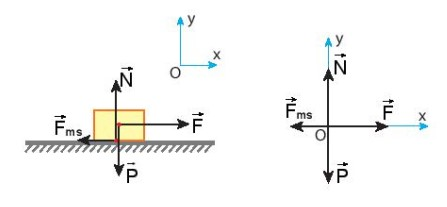
\includegraphics[scale=1]{../figs/VN10-2022-PH-TP021-1.jpg}
	\end{center}
	Thùng hàng chịu tác dụng của bốn lực: trọng lực $\vec P$, lực đẩy $\vec F$, phản ứng $\vec N$ và lực ma sát trượt $\vec F_\text{ms}$ của sàn.
	
	Áp dụng định luật II Newton:
	$$\overrightarrow{P}+\overrightarrow{N}+\overrightarrow{F}+\overrightarrow{F_{ms}}=m\vec{a}$$
	
	Chiếu phương trình định luật II Newton lên hệ trục $Oxy$:\\
	Trên trục $Ox$:
	\begin{equation}
		F - F_\text{ms} = ma_\text{x} = ma
	\end{equation}
	Trên trục $Oy$:
	\begin{equation}
		N - P = 0
	\end{equation}
	
	$$F_\text{ms} = \mu N.$$
	
	Giải hệ phương trình:
	
	$$N = mg = \SI{490}{N}.$$
	
	$$F_\text{ms} = \mu N = \SI{122,5}{N}.$$
	
	Gia tốc của vật:
	
	$$a = \dfrac{F - F_\text{ms}}{m} = \SI{1,15}{m/s}^2.$$
	
	Thùng hàng trượt với gia tốc $a = \SI{1,15}{m/s}^2$ cùng chiều với trục Ox.
	
	
	
}

\item \mkstar{3}


{Một người dùng dây buộc để kéo một thùng gỗ theo phương nằm ngang bằng một lực $\vec F$. Khối lượng của thùng $\SI{35}{kg}$. Hệ số ma sát giữa sàn và đáy thùng là 0,3. Lấy $g=\SI{9,8}{m/s}^2$.
	\begin{center}
		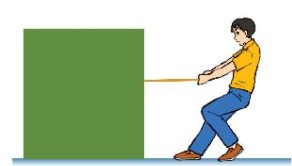
\includegraphics[scale=1]{../figs/VN10-2022-PH-TP021-2.jpg}
	\end{center}
	
	Tính độ lớn của lực kéo trong hai trường hợp:
	\begin{enumerate}[label=\alph*)]
		\item  Thùng trượt với gia tốc $\SI{0,2}{m/s}^2$.
		\item Thùng trượt đều.
	\end{enumerate}
}

\hideall
{
	\begin{center}
		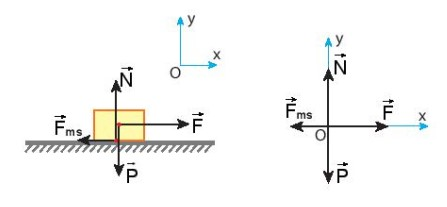
\includegraphics[scale=1]{../figs/VN10-2022-PH-TP021-1.jpg}
	\end{center}
	
	Coi thùng như một chất điểm và áp dụng định luật 2 Newton cho các lực thành phần theo các phương Ox, Oy.\\
	Trên $Ox$:
	\begin{equation}
		\label{eq:21-3}
		F - F_\text{ms} = ma_\text{x} = ma
	\end{equation}
	Trên $Oy$:
	\begin{equation}
		\label{eq:21-4}
		N - P =0
	\end{equation}
	$$F_\text{ms} = \mu N.$$
	
	Giải hệ phương trình:
	
	Từ (\ref{eq:21-4}) suy ra $N = mg$.
	
	Lực ma sát có giá trị:
	
	$$F_\text{ms} = \mu N = \mu mg.$$
	
	\begin{enumerate}[label=\alph*)]
		\item  Thùng trượt với gia tốc $\SI{0,2}{m/s}^2$
		
		$$F = m(a + \mu h) = \SI{109,9}{N}.$$
		\item Thùng trượt đều ($a =0$)
		
		$$F = \mu mg = \SI{102,9}{N}.$$
		
	\end{enumerate}
	
	
}
\end{enumerate}
